\chapter{Performance of Our Driver}
\label{chap:performance}
\todo{keep \cite{Traeger2008} in mind}

\section{First Virtual Machine Experiments}
\label{chap:performance.firstexperiments}
\todo{todo:} For testing purposes, we tried optimizing the performance by restricting support to AES256-XTS. This enabled removing some if-else constructs that dispatched de-/encryption functions based on whether AES128 or AES256 was used. Even though these conditionals were located in a performance critical section, we saw no speed improvements. Our theory for why this was the case is the following: our driver was only ever used for one LUKS2 partition and therefore always took the same path through the if-else (either always AES128 or always AES256). This trained the CPU's branch prediction on this one specific path. Thus, after a short training phase, the CPU always speculatively executed the correct path, resulting in the same performance as without the if-else.

\todo{todo:} The default compiler optimization settings in Visual Studio were a little bit conservative and also optimized for small code size rather than high speed/performance. After tuning these settings to enable more aggressive optimizations and also focus on speed rather than code size, we found that \todo{this is a little bit complicated...}.

\begin{figure}[htb!]
	\center
	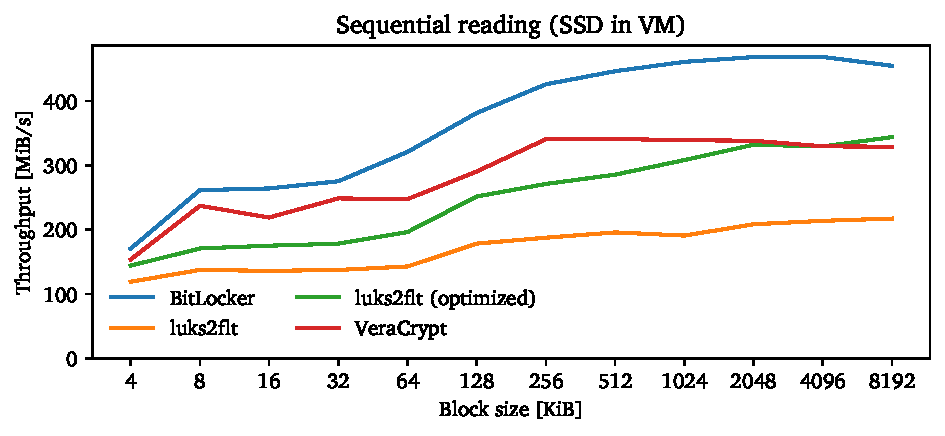
\includegraphics[scale=1]{../fig/performance.firstexperiments.seq.pdf}
	\caption[
		Comparison of sequential read throughput in a virtual machine
	]{
		Comparison of sequential read throughput in a virtual machine. \todo{todo}
	}
	\label{fig:performance.firstexperiments.rand}
\end{figure}

\begin{figure}[htb!]
	\center
	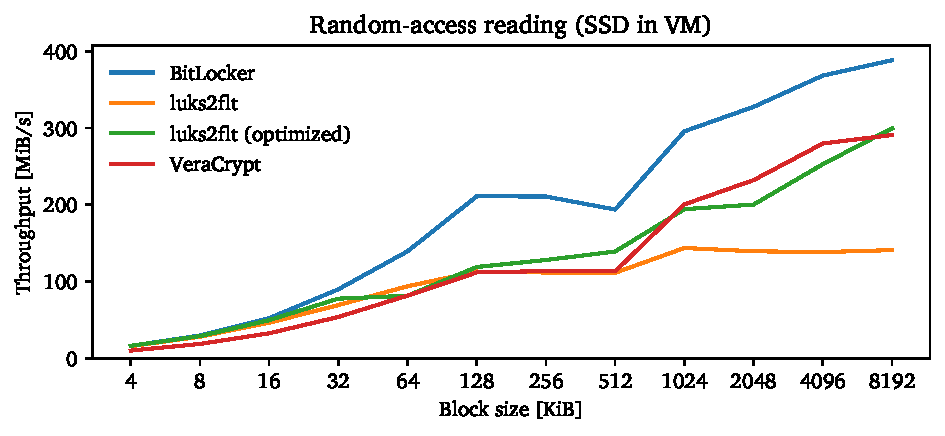
\includegraphics[scale=1]{../fig/performance.firstexperiments.rand.pdf}
	\caption[
		Comparison of random-access read throughput in a virtual machine
	]{
		Comparison of random-access read throughput in a virtual machine. \todo{todo}
	}
	\label{fig:performance.firstexperiments.rand}
\end{figure}

\section{Final Experimental Setup}
\label{chap:performance.finalsetup}
\begin{figure}[htb!]
	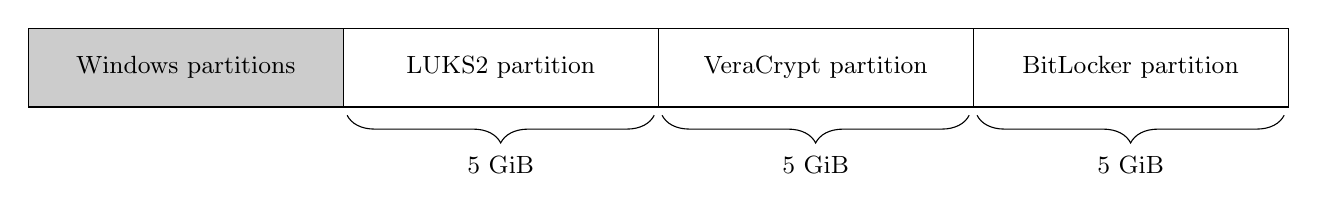
\begin{tikzpicture}
		\draw [fill={gray!40}] (0, 0) rectangle (4, 1);
		\node [anchor=center] at (2, 0.5) {\small\makecell{Windows partitions}};
		\draw [fill=white] (4, 0) rectangle (8, 1);
		\node [anchor=center] at (6, 0.5) {\small\makecell{LUKS2 partition}};
		\draw [fill=white] (8, 0) rectangle (12, 1);
		\node [anchor=center] at (10, 0.5) {\small\makecell{VeraCrypt partition}};
		\draw [fill=white] (12, 0) rectangle (16, 1);
		\node [anchor=center] at (14, 0.5) {\small\makecell{BitLocker partition}};

		\draw [decorate, decoration={brace, amplitude=10pt, mirror}, yshift=-3pt]
		(4.05, 0) -- (7.95, 0) node [black, midway, yshift=-18pt] {\small 5 GiB};
		\draw [decorate, decoration={brace, amplitude=10pt, mirror}, yshift=-3pt]
		(8.05, 0) -- (11.95, 0) node [black, midway, yshift=-18pt] {\small 5 GiB};
		\draw [decorate, decoration={brace, amplitude=10pt, mirror}, yshift=-3pt]
		(12.05, 0) -- (15.95, 0) node [black, midway, yshift=-18pt] {\small 5 GiB};
	\end{tikzpicture}
	\caption[
		Disk layout of the real hardware SSD
	]{
		Disk layout of the real hardware SSD.
	}
	\label{fig:performance.finalsetup.disklayoutssd}
\end{figure}

\todo{fio options, job files, and script}

\section{Results}
\label{chap:performance.results}

\subsection{Unencrypted Throughput Measurements}
\label{chap:performance.results.unencrypted}
\begin{figure}[htb!]
	\center
	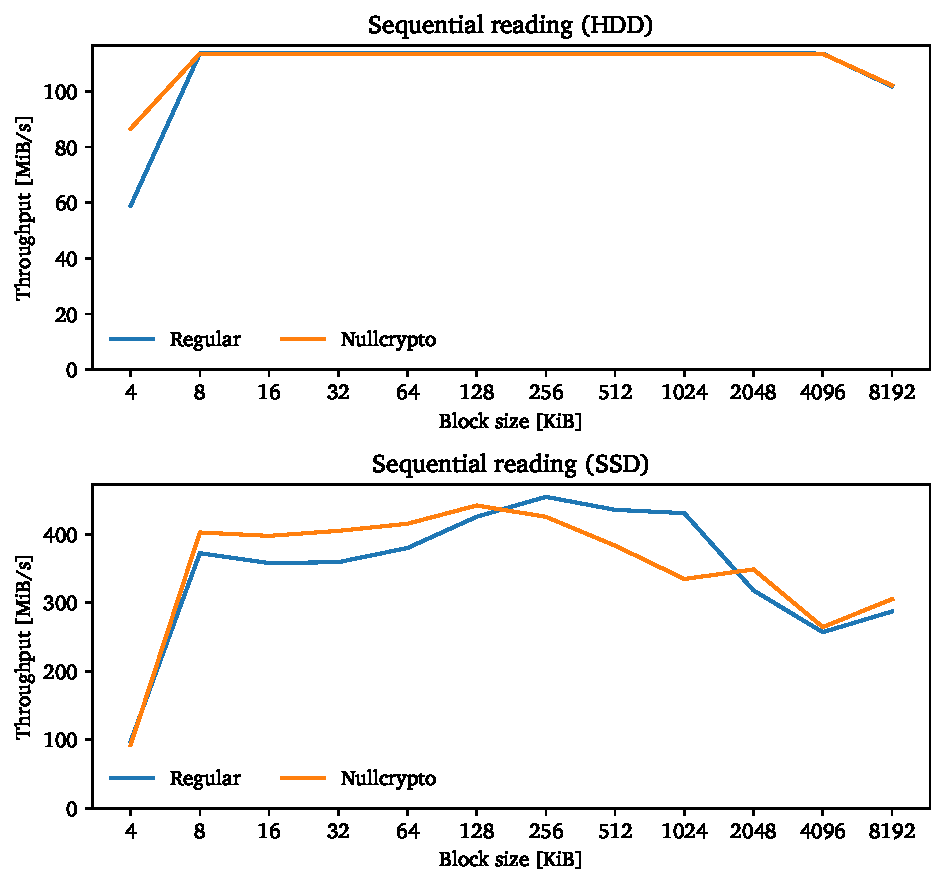
\includegraphics[scale=1]{../fig/performance.results.nullcryptoseq.pdf}
	\caption[
		Unencrypted versus null-crypto sequential read throughput
	]{
		Unencrypted versus null-crypto sequential read throughput. \todo{todo}
	}
	\label{fig:performance.results.nullcryptoseq}
\end{figure}

\begin{figure}[htb!]
	\center
	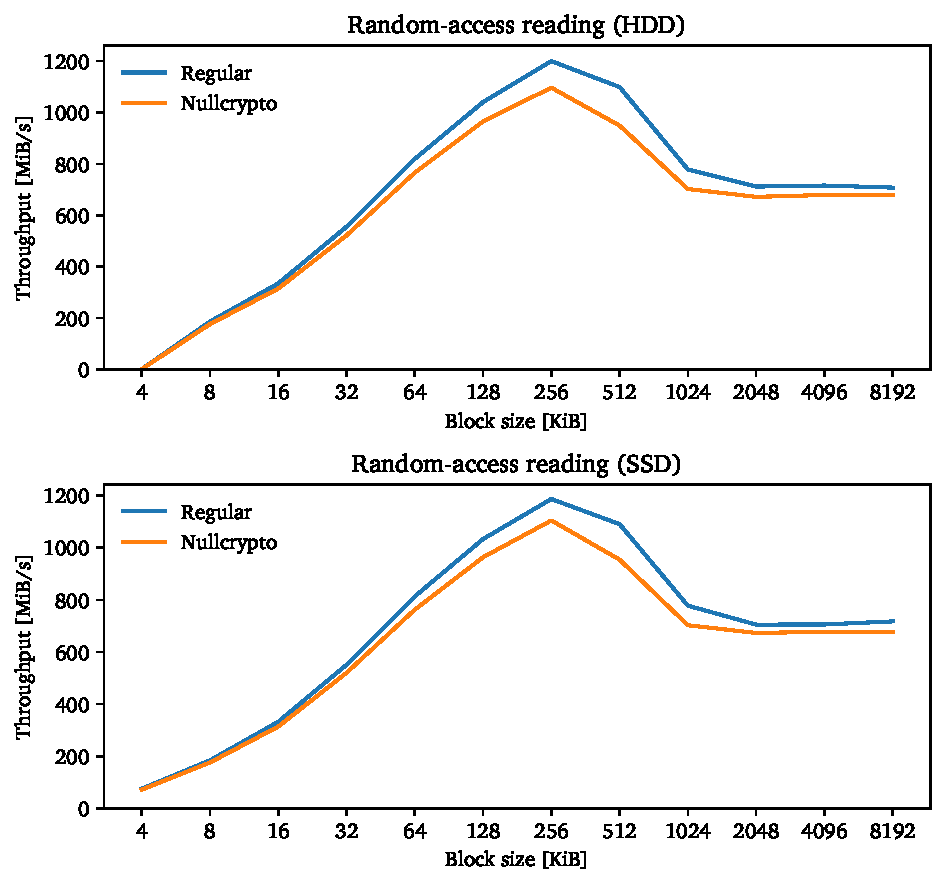
\includegraphics[scale=1]{../fig/performance.results.nullcryptorand.pdf}
	\caption[
		Unencrypted versus null-crypto random-access read throughput
	]{
		Unencrypted versus null-crypto random-access read throughput. \todo{todo}
	}
	\label{fig:performance.results.nullcryptorand}
\end{figure}

\subsection{First Series of Encrypted Throughput Measurements}
\label{chap:performance.results.encryptedseries1}
\begin{figure}[htb!]
	\center
	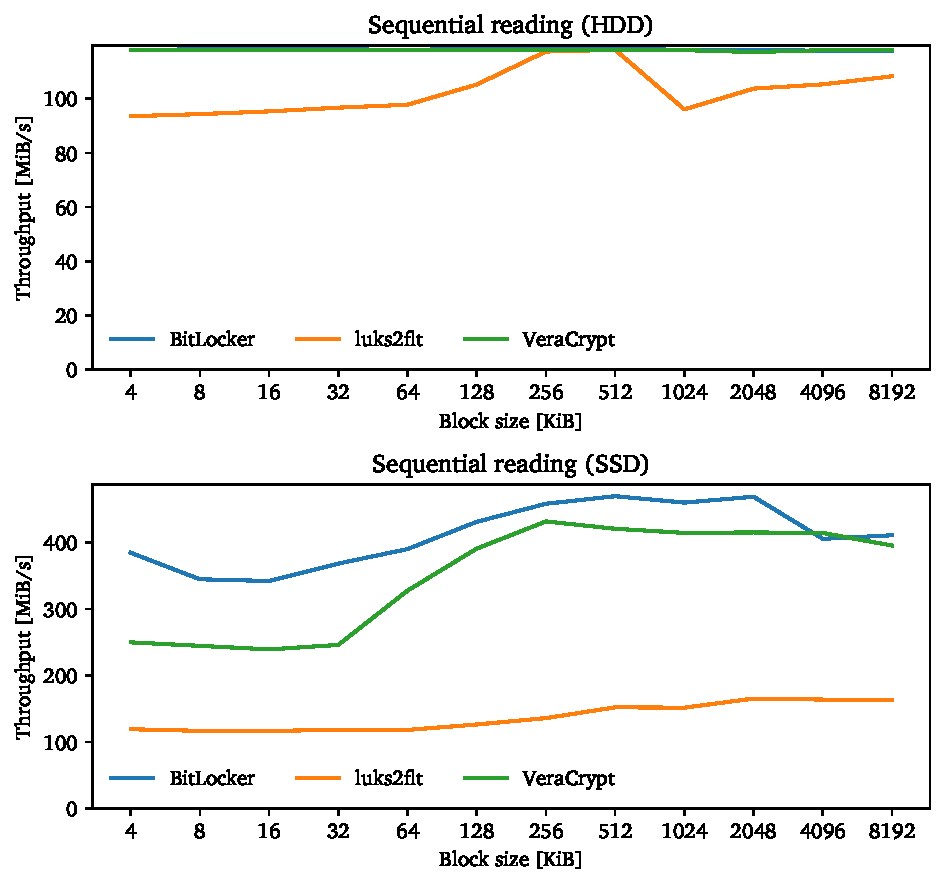
\includegraphics[scale=1]{../fig/performance.results.beforeoptseq.pdf}
	\caption[
		Comparison of sequential read throughput
	]{
		Comparison of sequential read throughput. \todo{todo}
	}
	\label{fig:performance.results.beforeoptseq}
\end{figure}

\begin{figure}[htb!]
	\center
	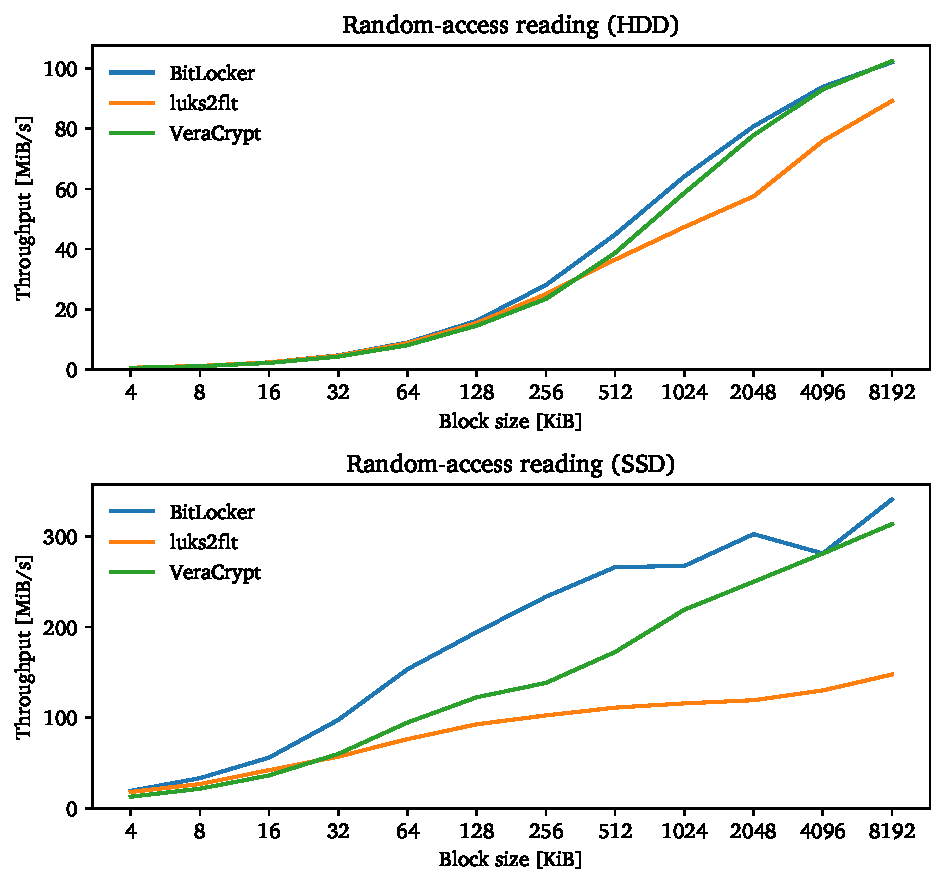
\includegraphics[scale=1]{../fig/performance.results.beforeoptrand.pdf}
	\caption[
		Comparison of random-access read throughput
	]{
		Comparison of random-access read throughput. \todo{todo}
	}
	\label{fig:performance.results.beforeoptrand}
\end{figure}

\subsection{Second Series of Encrypted Throughput Measurements}
\label{chap:performance.results.encryptedseries2}
\todo{all the different optimizedv2 graphs}

\begin{figure}[htb!]
	\center
	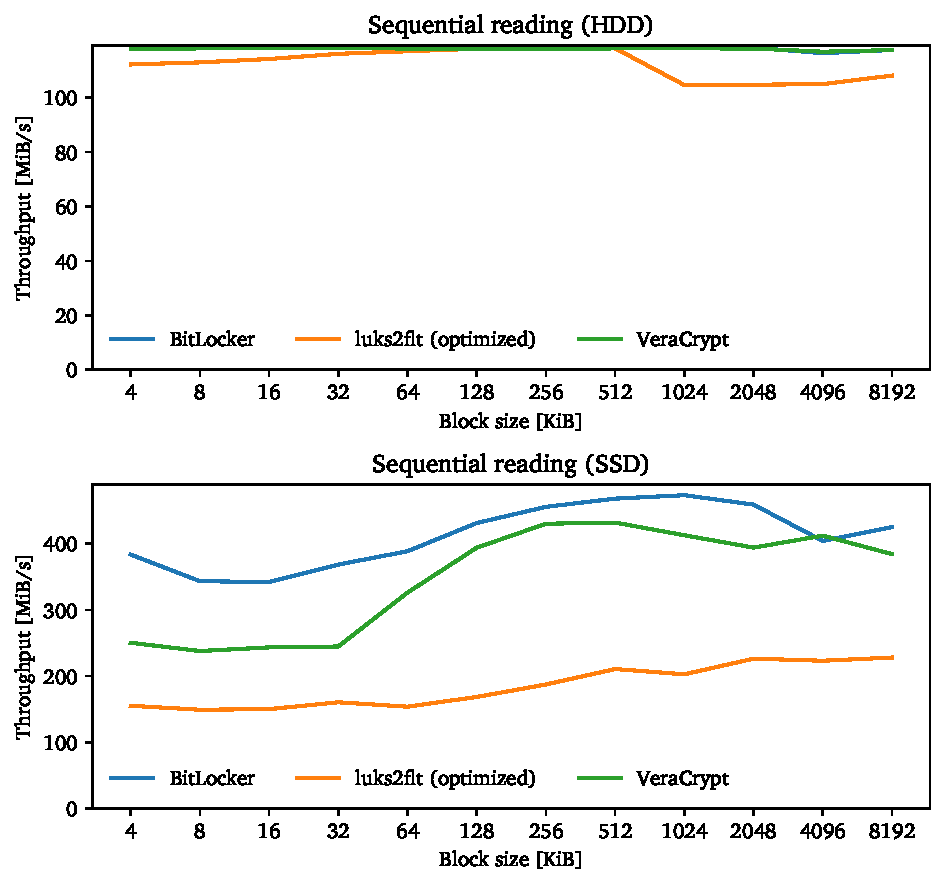
\includegraphics[scale=1]{../fig/performance.results.optseq.pdf}
	\caption[
		Comparison of sequential read throughput (optimized \texttt{luks2flt})
	]{
		Comparison of sequential read throughput (optimized \texttt{luks2flt}). \todo{todo}
	}
	\label{fig:performance.results.optseq}
\end{figure}

\begin{figure}[htb!]
	\center
	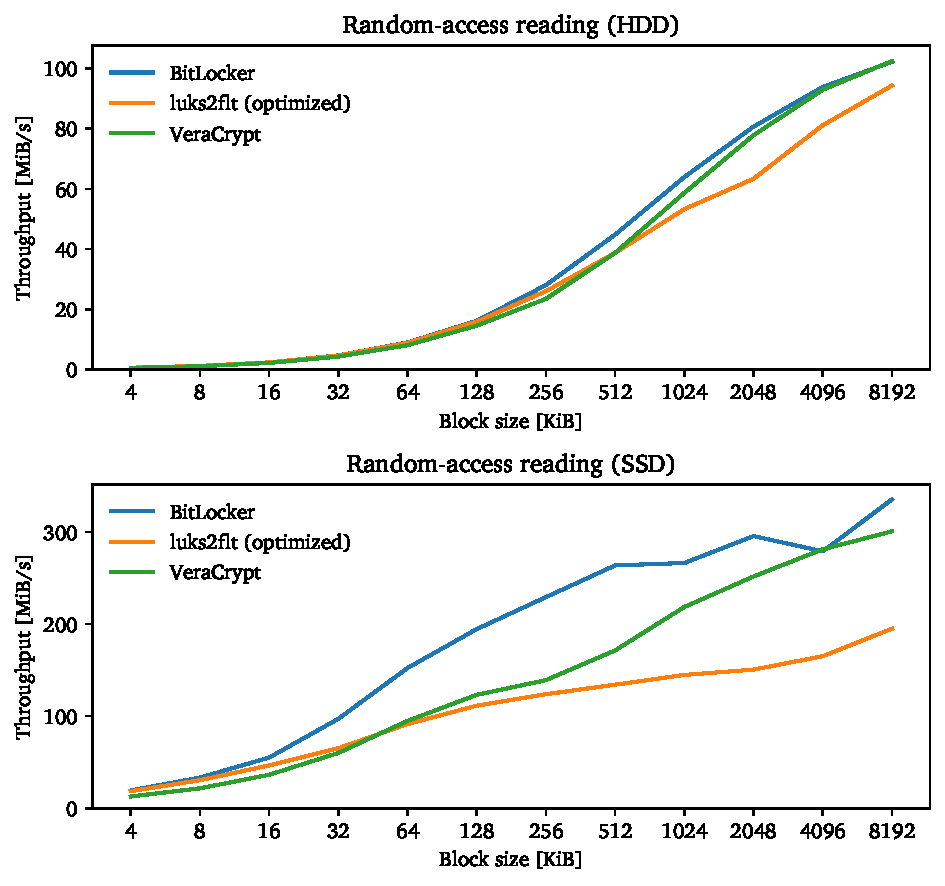
\includegraphics[scale=1]{../fig/performance.results.optrand.pdf}
	\caption[
		Comparison of random-access read throughput (optimized \texttt{luks2flt})
	]{
		Comparison of random-access read throughput (optimized \texttt{luks2flt}). \todo{todo}
	}
	\label{fig:performance.results.optrand}
\end{figure}

\begin{figure}[htb!]
	\center
	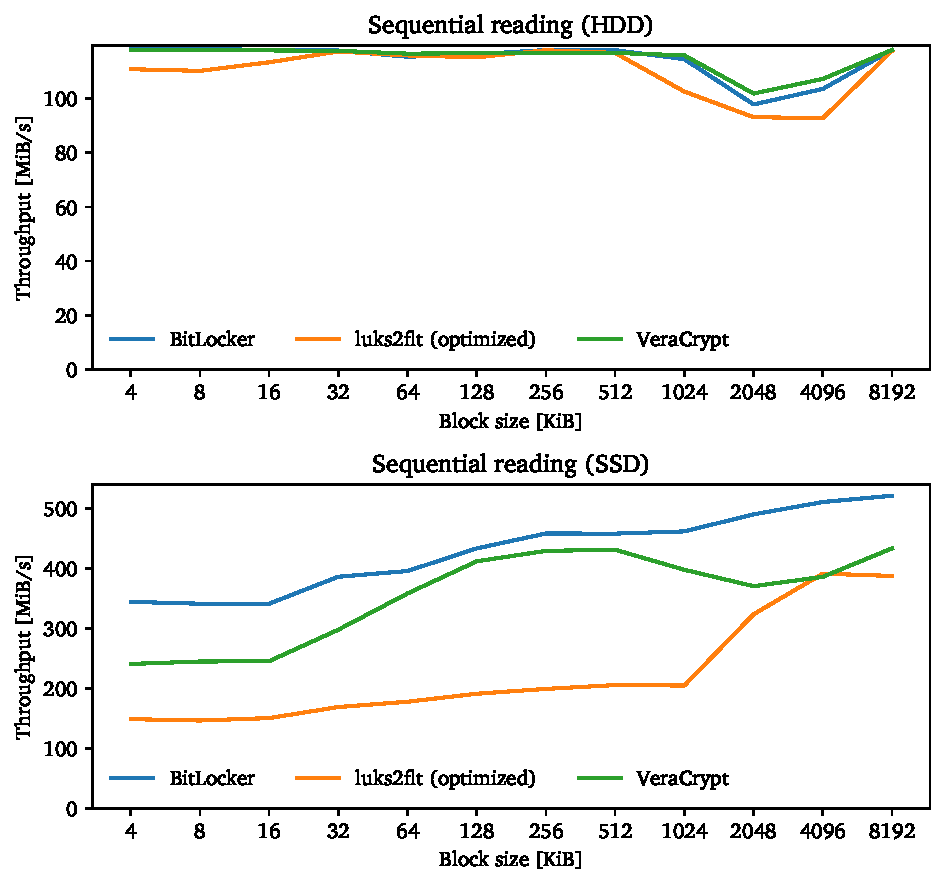
\includegraphics[scale=1]{../fig/performance.results.optseqqueue.pdf}
	\caption[
		Comparison of queued sequential read throughput (optimized \texttt{luks2flt})
	]{
		Comparison of queued sequential read throughput (optimized \texttt{luks2flt}). \todo{todo}
	}
	\label{fig:performance.results.optseqqueue}
\end{figure}

\begin{figure}[htb!]
	\center
	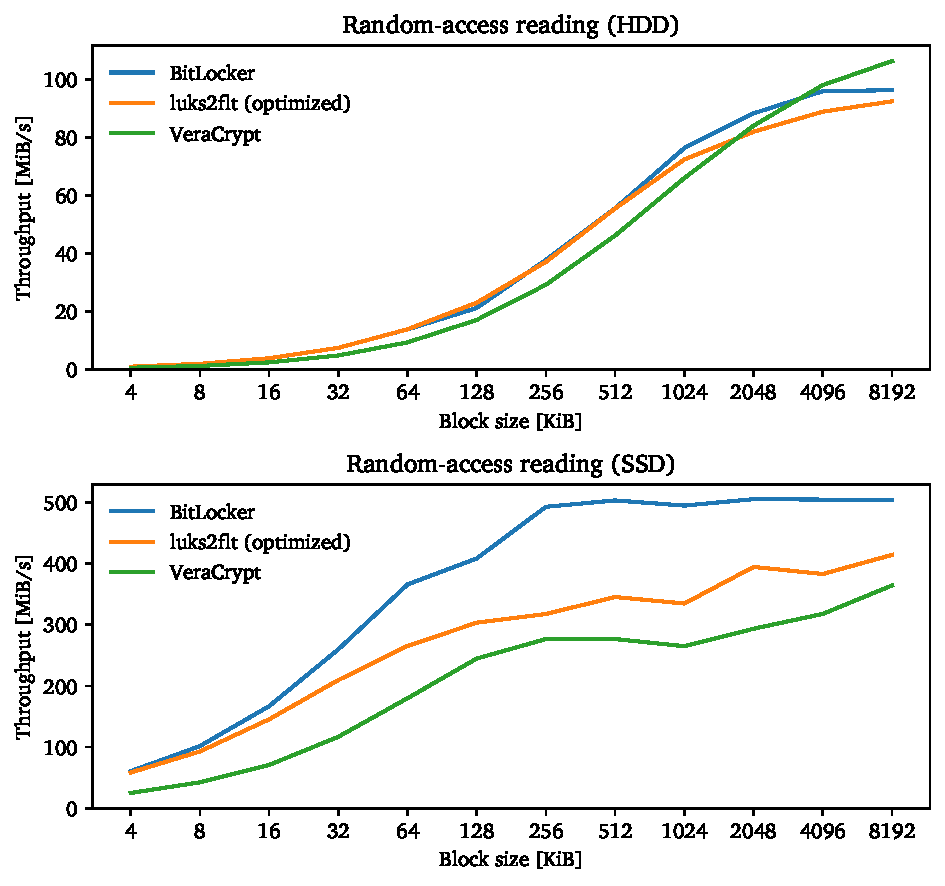
\includegraphics[scale=1]{../fig/performance.results.optrandqueue.pdf}
	\caption[
		Comparison of queued random-access read throughput (optimized \texttt{luks2flt})
	]{
		Comparison of queued random-access read throughput (optimized \texttt{luks2flt}). \todo{todo}
	}
	\label{fig:performance.results.optrandqueue}
\end{figure}

\begin{figure}[htb!]
	\center
	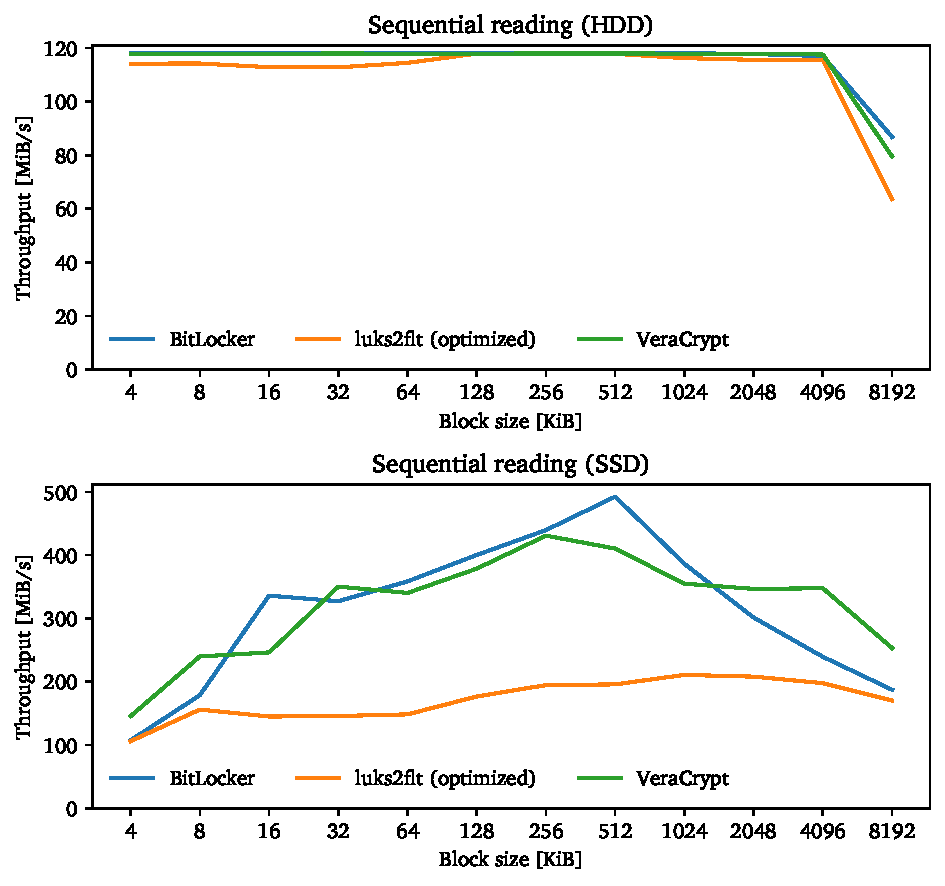
\includegraphics[scale=1]{../fig/performance.results.optseqthreads.pdf}
	\caption[
		Comparison of multi-threaded sequential read throughput (optimized \texttt{luks2flt})
	]{
		Comparison of multi-threaded sequential read throughput (optimized \texttt{luks2flt}). \todo{todo}
	}
	\label{fig:performance.results.optseqthreads}
\end{figure}

\begin{figure}[htb!]
	\center
	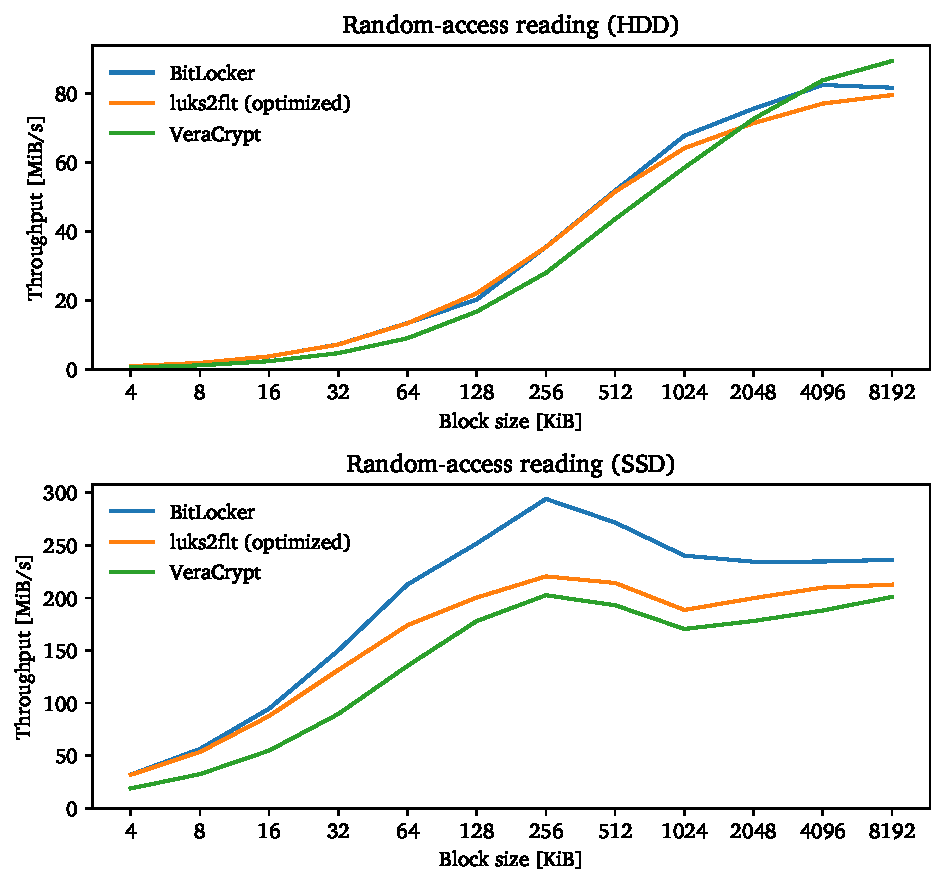
\includegraphics[scale=1]{../fig/performance.results.optrandthreads.pdf}
	\caption[
		Comparison of multi-threaded random-access read throughput (optimized \texttt{luks2flt})
	]{
		Comparison of multi-threaded random-access read throughput (optimized \texttt{luks2flt}). \todo{todo}
	}
	\label{fig:performance.results.optrandthreads}
\end{figure}

\begin{figure}[htb!]
	\center
	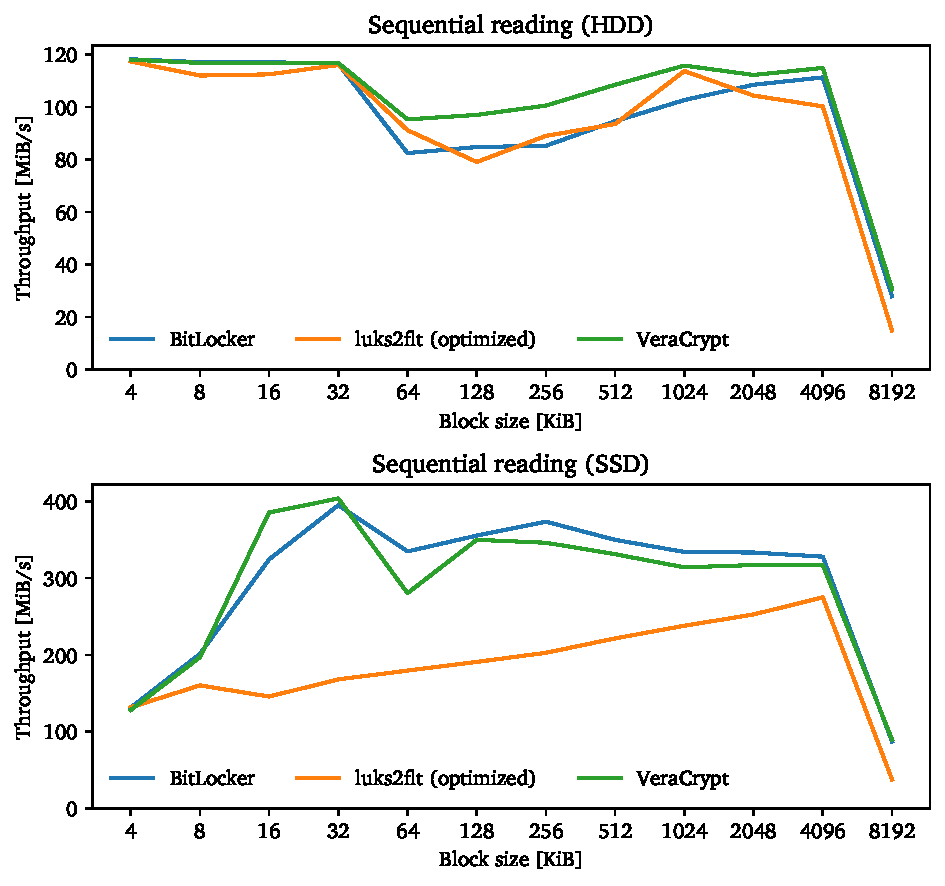
\includegraphics[scale=1]{../fig/performance.results.optseqthreadsqueue.pdf}
	\caption[
		Comparison of multi-threaded and queued sequential read throughput (optimized \texttt{luks2flt})
	]{
		Comparison of multi-threaded and queued sequential read throughput (optimized \texttt{luks2flt}). \todo{todo}
	}
	\label{fig:performance.results.optseqthreadsqueue}
\end{figure}

\begin{figure}[htb!]
	\center
	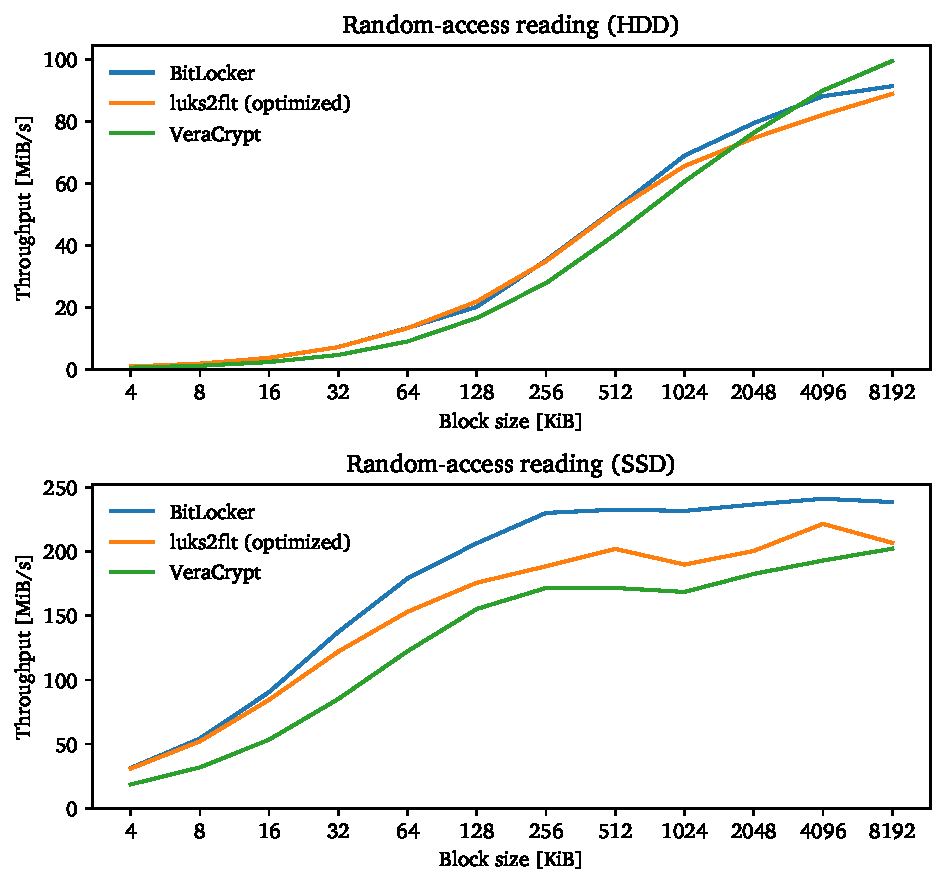
\includegraphics[scale=1]{../fig/performance.results.optrandthreadsqueue.pdf}
	\caption[
		Comparison of multi-threaded and queued random-access read throughput (optimized \texttt{luks2flt})
	]{
		Comparison of multi-threaded and queued random-access read throughput (optimized \texttt{luks2flt}). \todo{todo}
	}
	\label{fig:performance.results.optrandthreadsqueue}
\end{figure}

\subsection{Measuring Throughput Over Time}
\label{chap:performance.results.throughputovertime}
\todo{bw\_log graphs}